\documentclass[11pt,a4paper]{article}

\usepackage[utf8]{inputenc}
\usepackage[T1]{fontenc}
\usepackage[brazil]{babel}
\usepackage[margin=2cm]{geometry}
\usepackage{graphicx}
\usepackage{hyperref}
\usepackage{booktabs}
\usepackage{caption}
\usepackage{float}
\usepackage{subcaption}
\usepackage{microtype}

\hypersetup{
  colorlinks=true,
  linkcolor=black,
  urlcolor=blue,
  citecolor=black
}

\title{MC859 --- Teoria em Grafos \\ \large Entrega Parcial: Grafo de Colaborações entre Artistas}
\author{Cirilo Morais 168838}
\date{\today}

\begin{document}
\maketitle

\section{Introdução e coleta de dados}

Este projeto modela colaborações entre artistas musicais como um grafo
não direcionado, em que cada vértice representa um artista e cada
aresta representa o fato de dois artistas terem aparecido juntos como
créditos de uma mesma gravação. Cada aresta carrega como atributo o
peso $w_{uv}$ correspondente ao número de gravações compartilhadas pelos
dois artistas, e cada vértice carrega o nome do artista, o número total
de gravações em que aparece e (opcionalmente) seu gênero principal.

A coleta partiu da lista dos 100 artistas com mais ouvintes mensais dos Estados Unidos/Reino Unido no
Spotify, obtida do portal Chartmasters\footnote{\url{https://chartmasters.org/spotify-most-followed-artists/}},
usada como conjunto de \emph{seeds}. Inicialmente tentou-se obter o
catálogo de cada \emph{seed} diretamente da API oficial do Spotify, mas
essa abordagem foi descartada após sucessivos bloqueios por
\emph{rate limiting}: o volume de requisições necessário para enumerar
faixas e colaboradores de cada artista esgotava rapidamente a cota e
disparava \emph{cool down} prolongado, inviabilizando a coleta dentro
do prazo do projeto. Optou-se então pelo
\href{https://musicbrainz.org/doc/MusicBrainz_API}{MusicBrainz Web Service},
que oferece dados de créditos por gravação com licença aberta e uma
política de \emph{rate limiting} previsível (1 req/s). Para cada artista da
semente, o serviço foi consultado para resolver o MBID e paginar suas
gravações
(\texttt{/recording browse}). A coleta foi configurada para percorrer
todas as páginas disponíveis até um teto de 3000 gravações por artista
semente, mantendo todos os créditos secundários encontrados em cada
gravação. Após a coleta, gravações foram desduplicadas pela chave
\emph{(título normalizado, conjunto de MBIDs creditados)}, de modo que
versões \emph{live}, \emph{remaster} e EP de uma mesma colaboração
colapsem em uma única linha --- preserva-se a de \texttt{first-release-date}
mais antiga. Ao final, foram coletadas \textbf{66\,718 tracks}
únicas via MusicBrainz a partir das 100 \emph{seeds}, totalizando
$|V|=6\,874$ artistas distintos. As requisições à API do MusicBrainz
são limitadas a 1 req/s (política do serviço) e são armazenadas em um CSV.

A partir do CSV resultante, o grafo é montado adicionando uma aresta
entre cada par $(u,v)$ co-creditado em alguma gravação; arestas
repetidas incrementam o peso $w_{uv}$. Artistas seeds que não
colaboraram com ninguém ainda aparecem como vértices isolados.

\paragraph{Repositório.} Código, instâncias e figuras estão em
\url{https://github.com/cmmmf/MC859-Teoria-em-Grafos}. A instância
principal foi exportada em \textbf{GraphML} no caminho
\href{https://github.com/cmmmf/MC859-Teoria-em-Grafos/blob/main/internal/data/collab_graph.graphml}{\texttt{internal/data/collab\_graph.graphml}}.

\section{Análise inicial do grafo}

\subsection{Tamanho e grau médio}

A Tabela~\ref{tab:size} resume as estatísticas básicas da instância.
Por se tratar de um grafo simples não direcionado, vale
$\sum_{v\in V} \deg(v) = 2|E|$ e portanto o grau médio é
$\bar{d} = 2|E|/|V|$.

\begin{table}[H]
  \centering
  \begin{tabular}{lr}
    \toprule
    Métrica & Valor \\
    \midrule
    Número de vértices $|V|$        & 6\,874 \\
    Número de arestas  $|E|$        & 26\,955 \\
    Grau médio         $\bar{d}$    & 7{,}8426 \\
    Grau máximo                     & 1\,252 (Snoop Dogg) \\
    Grau mediano                    & 3 \\
    Vértices isolados ($\deg = 0$)  & 1 \\
    \bottomrule
  \end{tabular}
  \caption{Estatísticas básicas do grafo de colaborações.}
  \label{tab:size}
\end{table}

\subsection{Distribuição dos graus}

A Figura~\ref{fig:degree} mostra o histograma da distribuição de
graus do grafo, agrupando os graus em \emph{bins} de largura 10 e com
escala logarítmica no eixo~$y$. A distribuição é fortemente
cauda-pesada: a maioria dos vértices tem grau baixo (mediana 3) e uma
minoria de \emph{hubs} concentra colaborações --- consistente com o
comportamento esperado em redes de colaboração reais. Os 10 maiores
graus são, em ordem decrescente: Snoop Dogg (1252), Lil Wayne (623),
2Pac (447), Future (438), Chris Brown (408), Kendrick Lamar (387),
Eminem (373), Nicki Minaj (372), 50 Cent (327) e Dr. Dre (312).

\begin{figure}[H]
  \centering
  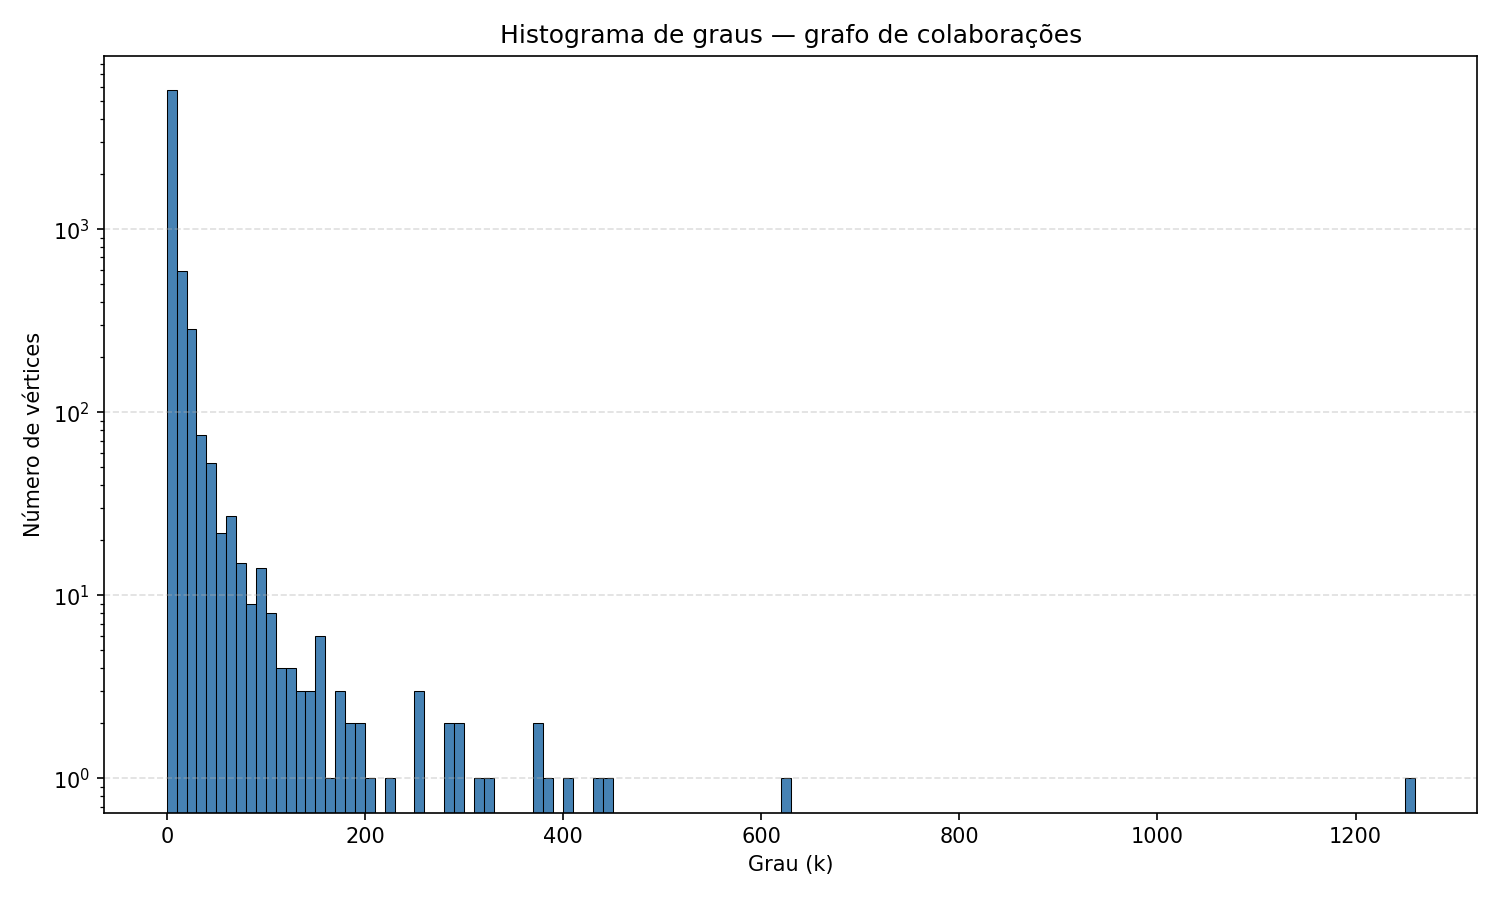
\includegraphics[width=0.85\linewidth]{figures/degree_distribution.png}
  \caption{Histograma da distribuição de graus do grafo. Eixo $y$ em
  escala logarítmica para acomodar a cauda longa.}
  \label{fig:degree}
\end{figure}

\subsection{Visualização do subgrafo dos 50 maiores hubs}

Visualizar o grafo completo ($|V|=6\,874$, $|E|=26\,955$) em uma figura
estática é pouco informativo: a quantidade de vértices e a densidade
da componente gigante saturam a imagem. Para tornar a estrutura
legível, a Figura~\ref{fig:top50} mostra apenas o subgrafo induzido
pelos 50 vértices de maior grau --- ou seja, os principais
\emph{hubs} da rede e as colaborações entre eles. Nessa escala fica
fácil identificar a comunidade de hip-hop/rap em torno de Snoop Dogg,
Lil Wayne e Eminem (vértices grandes e fortemente interligados) e
distingui-la de outros agrupamentos. O tamanho de cada vértice é
proporcional ao seu grau no subgrafo, a \textbf{cor representa o
gênero musical principal do artista} (obtido via MusicBrainz, com cor
estável por gênero) e a espessura das arestas é proporcional ao peso
$w_{uv}$ (número de colaborações entre os dois artistas).

\begin{figure}[H]
  \centering
  \includegraphics[width=0.9\linewidth]{figures/top50_graph.png}
  \caption{Subgrafo induzido pelos 50 artistas de maior grau no grafo
  de colaborações. Tamanho do vértice $\propto$ grau; cor $=$ gênero
  musical principal do artista; espessura da aresta $\propto$ número
  de colaborações.}
  \label{fig:top50}
\end{figure}

\subsection{Componentes conexas}

O grafo é não direcionado, então analisamos suas componentes conexas.
Foram identificadas \textbf{5 componentes conexas}, com a distribuição
de tamanhos da Tabela~\ref{tab:components}.

\begin{table}[H]
  \centering
  \begin{tabular}{rr}
    \toprule
    Tamanho da componente $k$ & Número de componentes \\
    \midrule
    1     & 1 \\
    2     & 1 \\
    3     & 1 \\
    4     & 1 \\
    6\,864 & 1 \\
    \bottomrule
  \end{tabular}
  \caption{Distribuição de tamanhos das componentes do grafo.}
  \label{tab:components}
\end{table}

A componente gigante cobre $6\,864/6\,874 \approx 99{,}85\%$ dos
vértices, restando apenas quatro pequenas componentes com 4, 3, 2 e 1
vértices respectivamente. É importante destacar que o grafo só possui
mais de uma componente conexa por um artefato da forma como ele foi
construído: a coleta partiu de apenas 100 \emph{seeds} (os artistas
com mais ouvintes mensais no Spotify) e expandiu somente por
co-créditos diretos dessas \emph{seeds}. Caso o universo completo de
artistas fosse considerado --- isto é, se a coleta fosse expandida
recursivamente a partir dos colaboradores de cada vértice já
incluído --- é muito provável que o grafo resultante tivesse uma
\emph{única} componente conexa, dado que todas as componentes pequenas
observadas aqui contêm artistas que claramente possuem colaborações
fora do nosso recorte (e.g. Black Sabbath, Led Zeppelin e The
Strokes têm cada um diversas colaborações com outros artistas que não
são \emph{seeds} e portanto não foram incluídos na coleta). As
componentes pequenas correspondem, portanto, a artistas cujos
colaboradores diretos ficaram fora do \emph{crawl} (e.g. \emph{Kanye
West Tribute Band} como único vértice; \emph{Black Sabbath, Keith
Moon, Led Zeppelin, The Strokes} como uma componente de tamanho 4).


\begin{figure}[H]
  \centering
  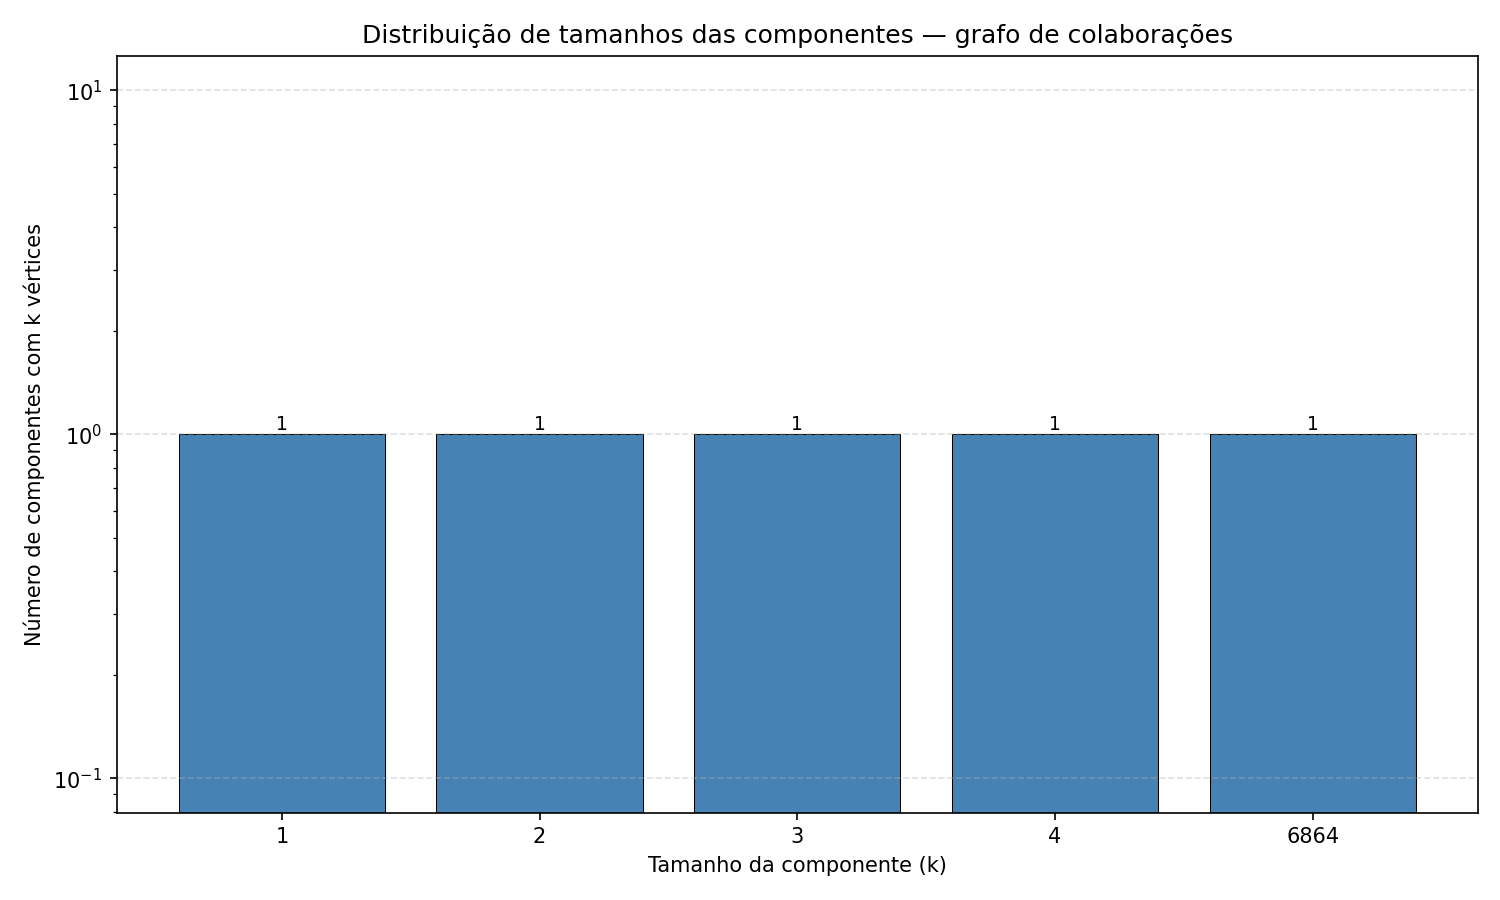
\includegraphics[width=0.7\linewidth]{figures/component_sizes.png}
  \caption{Distribuição dos tamanhos das componentes: número de
  componentes (eixo $y$, log) com $k$ vértices (eixo $x$).}
  \label{fig:components}
\end{figure}

\end{document}
